% Gemini theme
% https://github.com/anishathalye/gemini

\documentclass[final]{beamer}

% ====================
% Packages
% ====================

\usepackage[T1]{fontenc}
\usepackage{lmodern}
% \usepackage[size=custom,width=120,height=72,scale=1.0]{beamerposter}
\usepackage[size=B0]{beamerposter}
\usetheme{gemini}
\usecolortheme{gemini}
\usepackage{graphicx}
\usepackage{booktabs}
\usepackage{tikz}
\usepackage{rubikcube,rubikrotation,rubikpatterns,rubiktwocube}
\usepackage{multicol}

\usepackage{tikz-3dplot}
\usetikzlibrary{3d}

\usepackage{pgfplots}
\pgfplotsset{compat=1.14}
\usepackage{anyfontsize}

% ====================
% Lengths
% ====================

% If you have N columns, choose \sepwidth and \colwidth such that
% (N+1)*\sepwidth + N*\colwidth = \paperwidth
\newlength{\sepwidth}
\newlength{\colwidth}
\setlength{\sepwidth}{0.025\paperwidth}
\setlength{\colwidth}{0.3\paperwidth}

\newcommand{\separatorcolumn}{\begin{column}{\sepwidth}\end{column}}

% ====================
% Title
% ====================

\title{Understanding The Rubik's Cube: A Group Theoretic Approach}

% \author{Tony X \inst{1} \and Pesara A \inst{1} \and Zeyn J \inst{1}}
\author{Tony X \and Pesara A  \and Zeyn J}

%\institute[shortinst]{\inst{1} Some Institute \samelineand \inst{2} Another Institute}
% \institute[shortinst]{\inst{1} McMaster University}
% ====================
% Footer (optional)
% ====================

% \footercontent{
%  \href{https://www.github.com/PradCoder/4GR3Repository}{https://www.github.com/PradCoder/4GR3Repository} \hfill
%  ABC Conference 2025, New York --- XYZ-1234 \hfill}
%  \href{mailto:alyssa.p.hacker@example.com}{alyssa.p.hacker@example.com}}
% (can be left out to remove footer)

% ====================
% Logo (optional)
% ====================

% use this to include logos on the left and/or right side of the header:
% \logoright{\includegraphics[height=7cm]{logo1.pdf}}
% \logoleft{\includegraphics[height=7cm]{logo2.pdf}}

% ====================
% Body
% ====================

\begin{document}
\pgfmathsetmacro\radius{0.1}
\newcommand{\frontcolor}{red}
\newcommand{\sidecolor}{blue}
\begin{frame}[t]
\begin{columns}[t]
\separatorcolumn

\begin{column}{\colwidth}

  \begin{block}{Abstract}

  %  Some block contents, followed by a diagram, followed by a dummy paragraph.

%    \begin{figure}
%      \centering
%      \begin{tikzpicture}[scale=6]
%        \draw[step=0.25cm,color=gray] (-1,-1) grid (1,1);
%        \draw (1,0) -- (0.2,0.2) -- (0,1) -- (-0.2,0.2) -- (-1,0)
%          -- (-0.2,-0.2) -- (0,-1) -- (0.2,-0.2) -- cycle;
%      \end{tikzpicture}
%      \caption{A figure caption.}
  %  \end{figure}

    \textbf{The Rubik's Cube is perhaps the world's most famous puzzle and one that has caught the attention of many a mathematician.} 
    The first rigorous 
    mathematical analysis of a Rubik's Cube was done by British-American Mathemetician 
    David Singmaster, though solutions were known to a number of 
    mathematicians at the time (like J.H. Conway and Roger Penrose).  

    \textbf{In this project, we attempt to understand the inner workings of the Rubik's cube via group theory and abstract algebra.} 
    \begin{figure}[hbt]
    %\centering
    \RubikCubeSolved %Reset the cube configuration for use
    \RubikFaceUp   {R}{R}{R} {R}{R}{R} {R}{R}{R}%
    \RubikFaceFront {B}{B}{B} {B}{B}{B} {B}{B}{B}%
    \RubikFaceRight {W}{W}{W} {W}{W}{W} {W}{W}{W}%
    \RubikFaceDown {O}{O}{O} {O}{O}{O} {O}{O}{O}%
    \RubikFaceLeft {Y}{Y}{Y} {Y}{Y}{Y} {Y}{Y}{Y}%
    \RubikFaceBack  {G}{G}{G} {G}{G}{G} {G}{G}{G}%
    % \centering
    % \begin{multicols}{2}
      \centering
      % \begin{figure}
      \begin{tikzpicture}[z={(3.85mm,3.85mm)}]
          \DrawRubikCubeFlat
      \end{tikzpicture}
      % \end{figure}
      % \begin{figure}
      %   \centering
      %   $\Longleftrightarrow$%
      %   \centering
      % \end{figure}
      % \begin{figure}
      %   \centering
      %   \begin{tikzpicture}[z={(3.85mm,3.85mm)}]
      %     \DrawRubikCubeFlat
      %   \end{tikzpicture}
      % \end{figure}
      % \end{multicols}
      \caption{A flat map of the cube}
    \end{figure}
  \end{block}

  % \begin{block}{Modelling the Cube}


  % \end{block}

  \begin{alertblock}{Preliminary Definitions}


  \heading{Semi-direct products:}
     Let $G$ be a group with identity element $e$, a subgroup $H$ and a normal subgroup $N \triangleleft G$ such that $N \cap H = \{e\}$.
    Then the \textbf{semi-direct product} of $N$ and $H$ is $G = N \rtimes H$ if and only if for all $g \in G$ there exists a unique $n \in N$ and h \in H such that $g = nh$.
    %  \begin{enumerate}
    %   \item $G = NH$
    %   \item $N \cap H = e$
    %   \item $N \triangleleft K$
    %  \end{enumerate}

\heading{Wreath products:}

For $X$ be a finite set, $G$ a group and $H$ a group acting on $X$,
fix $\{x_1,x_2, \dots, x_t\}$, a labelling of $X$ with $| X | = t$ and 
let $G^t$ be the direct product of $G$ with itself $t$ times.
Then the \textbf{wreath product} of $G$ and $H$ is $G \wr H = G \rtimes H$ where $H$ acts on $G$ by its action on $X$.

% The wreath products of two groups $G$ and $H$ is constructed by: 
% \begin{enumerate}
% \item  Write $H$ as a permutation on $n$ items

% \item Make $n$ copies of the group $G$. $(G^n)$

% \item $H$ acts on the copies of $G$ by permuting the elements.
% \end{enumerate}

% The wreath product of $G$ by $H$ is a semi-direct product of a direct products of $n$ copies
% of $G$ by $H$.

% The wreath product permutes the factors of G according to the action h on X. So if $x \in G$, then the wreath product would take components of G and shuffle them around according to the action h on the set X.
    

\heading{Position Vectors:}
For any configuration of a Rubik's Cube there exists a corresponding \textbf{position vector} which is a $4$ tuple $(\rho, \sigma, v, w))$ where $\rho \in S_8, \sigma \in S_{12}$ describe the permutations of the cubies and $v \in \mathbb{Z}_3^8, w \in \mathbb{Z}_2^{12}$ describe the orientations of the cubies.

\textbf{Remark:} 
We will adopt Singmaster notation where  
we label the face with respect to it lying
flat on a plane and one is facing front face)

\begin{itemize}
\item Let $F$ denote the front face.
\item Let $L$ denote the left face.
\item Let $U$ denote the upward (top) face.
\item Let $D$ denote the downward (bottom) face.
\item Let $R$ denote the right face.
\item Let $B$ denote the back face.
\end{itemize}

\heading{Conjugates:}
For a group $G$ with $g,h \in G$, the \textbf{conjugate} of $g$ by $h$ is
$g^h = h^{-1}gh$ 

\heading{Commutators:}
For a group $G$ with $g,h \in G$ 
the \textbf{commutator} of $g$ and $h$ is 
$[g,h]=ghg^{-1}h^{-1}$

% The capital letter represent a $90\degree$ turn clockwise facing that face. The inverse of each move would be the $90\degree$ rotation of the face counter-clockwise (denoted by a $M^{-1}$ in our adaptation where $M$ \in \{F,L,U,D,R,B \}$).


    % This block catches your eye, so \textbf{important stuff} should probably go
    % here.

    % Curabitur eu libero vehicula, cursus est fringilla, luctus est. Morbi
    % consectetur mauris quam, at finibus elit auctor ac. Aliquam erat volutpat.
    % Aenean at nisl ut ex ullamcorper eleifend et eu augue. Aenean quis velit
    % tristique odio convallis ultrices a ac odio.

    % \begin{itemize}
    %   \item \textbf{Fusce dapibus tellus} vel tellus semper finibus. In
    %     consequat, nibh sed mattis luctus, augue diam fermentum lectus.
    %   \item \textbf{In euismod erat metus} non ex. Vestibulum luctus augue in
    %     mi condimentum, at sollicitudin lorem viverra.
    %   \item \textbf{Suspendisse vulputate} mauris vel placerat consectetur.
    %     Mauris semper, purus ac hendrerit molestie, elit mi dignissim odio, in
    %     suscipit felis sapien vel ex.
    % \end{itemize}

    % Aenean tincidunt risus eros, at gravida lorem sagittis vel. Vestibulum ante
    % ipsum primis in faucibus orci luctus et ultrices posuere cubilia Curae.

  \end{alertblock}
 
  \begin{block}{Relevant Theorems}

    \heading{Theorem on parity:} 
The cube always has even parity, or an even number of cubies
exchanged from the starting position.
%     Permutations can also be described in terms of their parity. Any length $n$-
% cycle of a permutation can be expressed as the product of $2$-cycles.

      \heading{Second Fundamental Theorem of Cubology: }
      An operation of the cube is possible if and only if:
            \begin{itemize}
              \item The total number of edge and corner cycles of even length is even.
              \item The number of corner cycles twisted right is equal to the number of corner cycles twisted left (up to modulo $3$).
              \item There is an even number of reorienting edge cycles.


    % $$
    % \int_{-\infty}^{\infty} e^{-x^2}\,dx = \sqrt{\pi}
    % $$

    % Interdum et malesuada fames $\{1, 4, 9, \ldots\}$ ac ante ipsum primis in
    % faucibus. Cras eleifend dolor eu nulla suscipit suscipit. Sed lobortis non
    % felis id vulputate.

    % \heading{Example of a semi direct product:}

    % The group $S_n$ can be written as a semi-direct product: $S_n =A_n \times \langle$

    % \heading{Another heading inside a block}

    % Sed augue erat, scelerisque a purus ultricies, placerat porttitor neque.
    % Donec $P(y \mid x)$ fermentum consectetur $\nabla_x P(y \mid x)$ sapien
    % sagittis egestas. Duis eget leo euismod nunc viverra imperdiet nec id
    % justo.

    \end{itemize}

  \end{block}
  


\end{column}

\begin{column}{\colwidth}

  \begin{alertblock}{The Fundamental Theorem of Cubology}
    
    \textbf{A move sequence is possible if and only if:} 
    % the following three conditions are satisfied, we also state the group theoretic formulation:

    \begin{enumerate}
      \item The permutation of the corner cubies has the same parity as the permutation of the edge cubies 
      % if and only if 
      $$\text{sign}(\rho) = \text{sign}(\sigma)$$
      \item The number of corners that are twisted clockwise is equal to the number that are twisted counterclockwise modulo $3$
      % (meaning remaining corners twisted in the same direction occur in threes).
      % if and only if 
      $$v_{1} + v_{2} +\dots +v_{8} \equiv 0 \mod 3$$
      \item The number of flipped edges is even
      % if and only if 
      $$w_{1} + w_{2} +\dots +w_{12} \equiv 0 \mod 2$$
    \end{enumerate}

  %  \textbf{Remark:}  We are considering the following defintion of a postion of a facet of a cube:
  %   A position vector $(\rho,\sigma,v,w) \in S_{8} \times S_{12} \times C_{3}^{8} \times C_{2}^{12}$

  \end{alertblock}

  \begin{block}{Proof of the Fundamental Theorem of Cubology (Summarized)}
    The Rubik's cube consists of $54$ facets and the entire set of arrangements of the Rubik's Cube are a subset of all possible permutations of these $54$ facets 
    denoted by the Rubik's Cube group i.e. $RC = \langle F,L,U,D,R,B\rangle \subset S_{54}$.

    % $$
    % \int_{-\infty}^{\infty} e^{-x^2}\,dx = \sqrt{\pi}
    % $$

    % Interdum et malesuada fames $\{1, 4, 9, \ldots\}$ ac ante ipsum primis in
    % faucibus. Cras eleifend dolor eu nulla suscipit suscipit. Sed lobortis non
    % felis id vulputate.

$(\implies)$ 
\textbf{We show that if $X$ is a legal configuration then the three conditions hold.}

Essentially, the six position vectors $(R,L,U,D,F,B)$ are perserved under these conditions.
$$F \rightarrow ((3, 7, 8, 4), (3, 7, 11, 8), (0, 0, 1, 2, 0, 0, 2, 1), (0, 0, 0, 0, 0, 0, 0, 0, 0, 0, 0, 0))$$
$$L \rightarrow ((1 ,4,8,5),(4,8,12,5),(2, 0, 0, 1, 1, 0, 0, 2), (0, 0, 0, 1, 1, 0, 0, 1, 0, 0, 0, 1))$$
$$U \rightarrow ((1, 2, 3, 4), (1, 2, 3, 4), (0, 0, 0, 0, 0, 0, 0, 0), (0, 0, 0, 0, 0, 0, 0, 0, 0, 0, 0, 0))$$
$$D \rightarrow ((5, 8, 7, 6), (9, 12, 11, 10), (0, 0, 0, 0, 0, 0, 0, 0), (0, 0, 0, 0, 0, 0, 0, 0, 0, 0, 0, 0))$$
$$R \rightarrow ((2,6,7,3),(2,6,10,7),(0,1,2,0,0,2,1,0),(0,1,0,0,0,1,1,0,0,1,0,0))$$
$$B \rightarrow ((1, 5, 6, 2), (1, 5, 9, 6), (1, 2, 0, 0, 2, 1, 0, 0), (0, 0, 0, 0, 0, 0, 0, 0, 0, 0, 0, 0))$$
Notice that each permutation is a $4$-cycle which is odd with sign $-1$, the sum of the component of each corner orientation vectors is either $0$ or $6$, both divisible by $3$ and 
the sum of the components of each edge orientation vector is either $0$ or $4$, both divisible by $2$.
% So every configuration obtained from these legal moves remains legal.

$(\impliedby)$ 
\textbf{We show that if the $3$ conditions hold then $X$ is a solvable configuration.}

For a legal configuration $X$ with position vector $(\rho, \sigma, v, w)$ assume that sign$(\rho)=$ sign$(\sigma)$.
% or apply a quarter turn to get the position vector mentioned above.
Notice that the corner cubies and the edge cubies have even parity so the corner cubies can be returned to their originial position by performing $3$-cycles on them. 
Call this configuration $X'$ with position vector $(\rho', \sigma', v', w')$.
Since $X$ satisfies the three conditions $X'$ also does with $\rho' = \epsilon$, $\sigma' = \epsilon$ because the solved state of the cube has position vector $(\epsilon, \epsilon, 0 , 0)$.

We can solve all edge cubies since we have moves to flip any pair of edges.
Now twist any clockwise or counterclockwise pairs to their original position.
Notice that all leftover corner twists occur in triplets, either all clockwise or all counterclockwise and are solvable with the corner twisting move.

% Therefore $X$ is a solvable configuration.

  \end{block}

  % \begin{block}{An algorithm for solving the Rubik's Cube}

  %   Nulla eget sem quam. Ut aliquam volutpat nisi vestibulum convallis. Nunc a
  %   lectus et eros facilisis hendrerit eu non urna. Interdum et malesuada fames
  %   ac ante \textit{ipsum primis} in faucibus. Etiam sit amet velit eget sem
  %   euismod tristique. Praesent enim erat, porta vel mattis sed, pharetra sed
  %   ipsum. Morbi commodo condimentum massa, \textit{tempus venenatis} massa
  %   hendrerit quis. Maecenas sed porta est. Praesent mollis interdum lectus,
  %   sit amet sollicitudin risus tincidunt non.

  %   Etiam sit amet tempus lorem, aliquet condimentum velit. Donec et nibh
  %   consequat, sagittis ex eget, dictum orci. Etiam quis semper ante. Ut eu
  %   mauris purus. Proin nec consectetur ligula. Mauris pretium molestie
  %   ullamcorper. Integer nisi neque, aliquet et odio non, sagittis porta justo.

  %   \begin{itemize}
  %     \item \textbf{Sed consequat} id ante vel efficitur. Praesent congue massa
  %       sed est scelerisque, elementum mollis augue iaculis.
  %       \begin{itemize}
  %         \item In sed est finibus, vulputate
  %           nunc gravida, pulvinar lorem. In maximus nunc dolor, sed auctor eros
  %           porttitor quis.
  %         \item Fusce ornare dignissim nisi. Nam sit amet risus vel lacus
  %           tempor tincidunt eu a arcu.
  %         \item Donec rhoncus vestibulum erat, quis aliquam leo
  %           gravida egestas.
  %       \end{itemize}
  %     \item \textbf{Sed luctus, elit sit amet} dictum maximus, diam dolor
  %       faucibus purus, sed lobortis justo erat id turpis.
  %     \item \textbf{Pellentesque facilisis dolor in leo} bibendum congue.
  %       Maecenas congue finibus justo, vitae eleifend urna facilisis at.
  %   \end{itemize}

  % \end{block}

  \begin{block}{Constructing the Legal Rubik's Cube Group}
    

    % The Rubik's Cube group can be "partitioned" into two major subgroups: 
    % the Illegal Rubik's Cube Group and the Legal Rubik's Cube group where the Legal Rubik's Cube group is a subgroup of the Illegal Rubik's Cube group.
    % Unlike the Legal Rubik's Cube Group, the Illegal Rubik's Cube Group allows the solver to take the cube apart and rearrange the facets.  

    % From the description of the corner and edge cubes, we can see that the 
    
    The Illegal Rubik's Cube group is:
    $$IRC_{3} = (\mathbb{Z}^{12}_2 \wr S_{12}) \times (\mathbb{Z}^8_3 \wr S_8)$$
    $$|IRC_{3}| = 2^{12} \times 12! \times 3^8 \times 8! = 519024039293878272000$$
    
\begin{itemize} 
\item The corner facets are represented by cyclic group of 3 elements $\mathbb{Z}_{3}$ and since there are $8$ copies we denote it by $\mathbb{Z}_3 ^8$.
\item The possible arrangements of the corner cubes are represented by $S_{8}$ (since we are permuting those), and postions of all the corner facets are represented by $\mathbb{Z}_{3}^{8} \wr S_{8}$.
\item Using a similar argument, the position of all the edge facets on the Rubik's Cube are represented by the group $\mathbb{Z}_{12}^{2} \wr S_{12}$.
\end{itemize} 

    \textbf{The Legal Rubik's Cube group is a subgroup of the Illegal Rubik's Cube Group because there are configurations of the cube that cannot be realized by only using the rotaions.}
$$LRC_{3} \approx (\mathbb{Z}_{3}^{7} \wr S_{8}) \times (\mathbb{Z}_{2}^{10} \wr S_{12}) \subset  (\mathbb{Z}^{12}_2 \wr S_{12}) \times (\mathbb{Z}^8_3 \wr S_8) \approx RC^{*}_{3}$$
$$ |LRC_{3}| = 2^{10} \times 12! \times 3^7 \times 8! = 43252003274489856000$$

% $$RC_{3} \cong (C_{3}^{7} \wr S_{8}) \times (C_{2}^{10} \wr S_{12})\subset (C_{3}^{7} \wr S_{8}) \times (C_{2}^{11} \wr S_{12}) \subset RC_{3}^{*} \cong C_{2}^{12} \times S_{8} \times C_{3}^{8} \times S_{8} \times S_{8}\subset S_{54}$$
    % \heading{Construction of the illegal Rubik's cube:}

    % First we construct the illegal Rubik's cube group since the legal Rubik's cube group is a subgroup of the illegal Rubik's cube group.
    
    % We also notice that the Rubik's cube group is a subgroup of the illegal rubik's cube group.


    % \heading{Construction of the legal Rubik's cube}

    % Now, we will construct the legal Rubik's cube.

    

% Now note that not all arrangments of the permutations would lead to the valid arrangements of a rubik's cube, 



  \end{block}

\end{column}

\separatorcolumn

\begin{column}{\colwidth}

  \begin{block}{Unsolvable Cubes}

    These cubes are unsolvable since they involve odd permutations.

    \begin{enumerate}
      
      \item \textbf{Exactly one edge cubie is flipped:}
      A singular edge cubie flipped 90 degrees is not possible since the cube always has even parity.
      
    \tdplotsetmaincoords{55}{135}
    \begin{figure}
      \centering
      \RubikFaceUp   {R}{R}{R} {R}{R}{R} {R}{B}{R}%
      \RubikFaceFront {B}{R}{B} {B}{B}{B} {B}{B}{B}%
      \RubikFaceRight {W}{W}{W} {W}{W}{W} {W}{W}{W}%
      \RubikFaceDown {O}{O}{O} {O}{O}{O} {O}{O}{O}%
      \RubikFaceLeft {Y}{Y}{Y} {Y}{Y}{Y} {Y}{Y}{Y}%
      \RubikFaceBack  {G}{G}{G} {G}{G}{G} {G}{G}{G}%
        \begin{tikzpicture}[z={(3.85mm,3.85mm)}]
        \DrawRubikCubeRU
        \end{tikzpicture}
      \caption{One edge cubie is flipped}
    \end{figure}
    
        
      \item \textbf{Corner twist:}
      A singular twisted corner is an impossible case since
      the cube always has even parity 
      and a corner twist is an odd permutation.
      \begin{figure}
        \centering
                \RubikFaceUp   {R}{R}{R} {R}{R}{R} {R}{R}{W}%
                \RubikFaceFront {B}{B}{R} {B}{B}{B} {B}{B}{B}%
                \RubikFaceRight {B}{W}{W} {W}{W}{W} {W}{W}{W}%
                \RubikFaceDown {O}{O}{O} {O}{O}{O} {O}{O}{O}%
                \RubikFaceLeft {Y}{Y}{Y} {Y}{Y}{Y} {Y}{Y}{Y}%
                \RubikFaceBack  {G}{G}{G} {G}{G}{G} {G}{G}{G}%
                  \begin{tikzpicture}[z={(3.85mm,3.85mm)}]
                  \DrawRubikCubeRU
                  \end{tikzpicture}
                  \caption{Corner twist}
                \end{figure}
           
                                                      

      \item \textbf{Swapped pieces:}
      For both edge and corner pieces, exactly two adjacent or opposite pieces cannot be swapped.
      \begin{figure}
        \centering
        \begin{multicols}{4}  
          \centering
          \RubikFaceUp   {R}{R}{R} {R}{R}{R} {R}{R}{R}%
          \RubikFaceFront {B}{G}{B} {B}{B}{B} {B}{B}{B}%
          \RubikFaceRight {W}{W}{W} {W}{W}{W} {W}{W}{W}%
          \RubikFaceDown {O}{O}{O} {O}{O}{O} {O}{O}{O}%
          \RubikFaceLeft {Y}{Y}{Y} {Y}{Y}{Y} {Y}{Y}{Y}%
          \RubikFaceBack  {G}{B}{G} {G}{G}{G} {G}{G}{G}%
          \begin{tikzpicture}[z={(3.85mm,3.85mm)}]
            \DrawRubikCubeRU
          \end{tikzpicture}

          \centering
          \RubikFaceUp   {R}{R}{R} {R}{R}{R} {R}{R}{R}%
          \RubikFaceFront {B}{W}{B} {B}{B}{B} {B}{B}{B}%
          \RubikFaceRight {W}{B}{W} {W}{W}{W} {W}{W}{W}%
          \RubikFaceDown {O}{O}{O} {O}{O}{O} {O}{O}{O}%
          \RubikFaceLeft {Y}{Y}{Y} {Y}{Y}{Y} {Y}{Y}{Y}%
          \RubikFaceBack  {G}{G}{G} {G}{G}{G} {G}{G}{G}%
            \begin{tikzpicture}[z={(3.85mm,3.85mm)}]
            \DrawRubikCubeRU
            \end{tikzpicture}

          \centering
          \RubikFaceUp   {R}{R}{R} {R}{R}{R} {R}{R}{R}%
          \RubikFaceFront {B}{B}{W} {B}{B}{B} {B}{B}{B}%
          \RubikFaceRight {G}{W}{B} {W}{W}{W} {W}{W}{W}%
          \RubikFaceDown {O}{O}{O} {O}{O}{O} {O}{O}{O}%
          \RubikFaceLeft {Y}{Y}{Y} {Y}{Y}{Y} {Y}{Y}{Y}%
          \RubikFaceBack  {W}{G}{G} {G}{G}{G} {G}{G}{G}%
            \begin{tikzpicture}[z={(3.85mm,3.85mm)}]
            \DrawRubikCubeRU
            \end{tikzpicture}
          
          \centering
          \RubikFaceUp   {R}{R}{R} {R}{R}{R} {R}{R}{R}%
          \RubikFaceFront {B}{B}{G} {B}{B}{B} {B}{B}{B}%
          \RubikFaceRight {Y}{W}{W} {W}{W}{W} {W}{W}{W}%
          \RubikFaceDown {O}{O}{O} {O}{O}{O} {O}{O}{O}%
          \RubikFaceLeft {W}{Y}{Y} {Y}{Y}{Y} {Y}{Y}{Y}%
          \RubikFaceBack  {G}{G}{B} {G}{G}{G} {G}{G}{G}%
            \begin{tikzpicture}[z={(3.85mm,3.85mm)}]
            \DrawRubikCubeRU
            \end{tikzpicture}
    \end{multicols}
    \caption{Swapped pieces}
  \end{figure}
    \end{enumerate}

                       

    % \begin{figure}
    %   \centering
    %   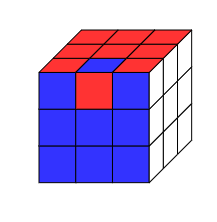
\includegraphics{Screenshot from 2024-03-26 11-14-42.png}
    %   \caption{One edge cubie is flipped}
    % \end{figure}

  \end{block}

  \begin{alertblock}{How does this relate to MATH 4GR3?}

    % \heading{Commutators and Conjugates}

    \textbf{When analyzing permutations, certain moves sequences are more effective than others like moves done by commutators.}

    If $y$ and $h$ are moves that fail to commute with each other by "just a little bit",
    then $[y,h]$ will be close to the identity (i.e. the solved state). 
    
    For a permutation $\alpha \in RC$ define $\text{fix}(\alpha)$ to be the set of all cubies that are not moved and
    the set of cubies moved as the support of $\alpha$ (denoted $\text{supp}(\alpha)$):  
    $$\text{supp}(\alpha) = \overline{\text{fix}(\alpha)} = \{m \in \text{cubies} : \alpha(m) \neq m\}$$

    \textbf{Commutators provide us with a method for creating puzzles moves that affect a small number of pieces and Conjugation is a process for modifying the moves of the commutators to produce new moves that have similar structure}.

    \begin{figure}
      \centering
      \begin{multicols}{2}  
        \centering
        \RubikFaceUp   {R}{R}{R} {R}{R}{R} {Y}{R}{W}%
        \RubikFaceFront {R}{B}{R} {B}{B}{B} {B}{B}{B}%
        \RubikFaceRight {B}{W}{W} {W}{W}{W} {W}{W}{W}%
        \RubikFaceDown {O}{O}{O} {O}{O}{O} {O}{O}{O}%
        \RubikFaceLeft {Y}{Y}{B} {Y}{Y}{Y} {Y}{Y}{Y}%
        \RubikFaceBack  {G}{G}{G} {G}{G}{G} {G}{G}{G}%
        \begin{tikzpicture}[z={(3.85mm,3.85mm)}]
          \DrawRubikCubeFlat
        \end{tikzpicture}
        
        \centering
        \RubikFaceUp   {R}{R}{G} {R}{R}{R} {Y}{R}{R}%
        \RubikFaceFront {R}{B}{B} {B}{B}{B} {B}{B}{B}%
        \RubikFaceRight {W}{W}{R} {W}{W}{W} {W}{W}{W}%
        \RubikFaceDown {O}{O}{O} {O}{O}{O} {O}{O}{O}%
        \RubikFaceLeft {Y}{Y}{B} {Y}{Y}{Y} {Y}{Y}{Y}%
        \RubikFaceBack  {W}{G}{G} {G}{G}{G} {G}{G}{G}%
          \begin{tikzpicture}[z={(3.85mm,3.85mm)}]
          \DrawRubikCubeFlat
          \end{tikzpicture}
  \end{multicols}
  \caption{$x = [LD^{2}L^{-1}F^{-1}D^{2}F,U]$ twists adjacent corners can be conjugated as $R^{x}$ which twists opposite corners}
\end{figure}
    % \item 
    % In the Rubik's Cube group we have the following commutator for instance, followed by a commutator that
    % can be used to adjust the move done by the commutator by changing the elements permuted, the type (structure on the move) is essentially
    % the same but different pieces are moved
    % In permutation puzzles $mov(\alpha)$ is the list of all the positions of the pieces that are moved when $\alpha$ is applied.

    % \begin{table}
    %   \centering
    %   \begin{tabular}{l r r c}
    %     \toprule
    %     \textbf{First column} & \textbf{Second column} & \textbf{Third column} & \textbf{Fourth} \\
    %     \midrule
    %     Foo & 13.37 & 384,394 & $\alpha$ \\
    %     Bar & 2.17 & 1,392 & $\beta$ \\
    %     Baz & 3.14 & 83,742 & $\delta$ \\
    %     Qux & 7.59 & 974 & $\gamma$ \\
    %     \bottomrule
    %   \end{tabular}
    %   \caption{A table caption.}
    % \end{table}

  \end{alertblock}

  \begin{block}{References}

    \nocite{*}
    \footnotesize{\bibliographystyle{ieeetr}\bibliography{poster}}

  \end{block}

\end{column}

\separatorcolumn
\end{columns}
\end{frame}

\end{document}